\documentclass[landscape]{article}
\setlength\textwidth{10in}
\setlength\textheight{8.5in}
\setlength\oddsidemargin{-.5in}
\setlength\evensidemargin{-.5in}
\setlength\topmargin{-.7in}
\setlength\headsep{0in}
\setlength\headheight{0in}
\setlength\topskip{0in}
\usepackage{tikz-qtree-compat}
\usepackage{spverbatim}
\usepackage{amssymb}
\usepackage{rotating}
\usepackage{color}
\usepackage{environ}
\usepackage{graphicx}
\usepackage{calc}

\newlength{\xsize}
\newlength{\ysize}
\newsavebox{\tempbox}

\newcommand{\maxsize}[1]{
  \savebox{\tempbox}{#1}
  \settoheight{\ysize}{\usebox{\tempbox}}
  \settowidth{\xsize}{\usebox{\tempbox}}
  \pgfmathparse{\xsize/\textwidth > \ysize/\textheight}
  \if \pgfmathresult1
    \resizebox{\textwidth}{!}{\usebox{\tempbox}}
  \else
    \resizebox{!}{\textheight-2cm}{\usebox{\tempbox}}
  \fi
}

\begin{document}
  \begin{spverbatim}
    15 (211, p, yes): Two dogs are playing by a tree
  \end{spverbatim}
  \noindent\maxsize{\begin{tikzpicture}[grow=down]
    \tikzset{level distance = 25pt, sibling distance = -5pt}
    \tikzset{every tree node/.style={align=center,anchor=north}}
    \Tree
      [. \node{${\tt ba}[s\!:\!dcl]$};
        [. \node{${\tt lx}[np, n]$};
          [. \node{${\tt fa}[n]$};
            [. \node{\begin{tabular}{c}
            \texttt{Two}\\
            $n/n$ \\
            \textbf{two}\\
            \normalsize{CD}\\
            \scriptsize{I-NP}\\
            \scriptsize{O}\\
            \end{tabular} }; ]
            [. \node{\begin{tabular}{c}
            \texttt{dogs}\\
            $n$ \\
            \textbf{dog}\\
            \normalsize{NNS}\\
            \scriptsize{I-NP}\\
            \scriptsize{O}\\
            \end{tabular} }; ]
          ]
        ]
        [. \node{${\tt fa}[s\!:\!dcl\backslash np]$};
          [. \node{\begin{tabular}{c}
          \texttt{are}\\
          $(s\!:\!dcl\backslash np)/(s\!:\!ng\backslash np)$ \\
          \textbf{be}\\
          \normalsize{VBP}\\
          \scriptsize{I-VP}\\
          \scriptsize{O}\\
          \end{tabular} }; ]
          [. \node{${\tt ba}[s\!:\!ng\backslash np]$};
            [. \node{\begin{tabular}{c}
            \texttt{playing}\\
            $s\!:\!ng\backslash np$ \\
            \textbf{play}\\
            \normalsize{VBG}\\
            \scriptsize{I-VP}\\
            \scriptsize{O}\\
            \end{tabular} }; ]
            [. \node{${\tt fa}[(s\!:\!ng\backslash np)\backslash (s\!:\!ng\backslash np)]$};
              [. \node{\begin{tabular}{c}
              \texttt{by}\\
              $((s\!:\!ng\backslash np)\backslash (s\!:\!ng\backslash np))/np$ \\
              \textbf{by}\\
              \normalsize{IN}\\
              \scriptsize{I-PP}\\
              \scriptsize{O}\\
              \end{tabular} }; ]
              [. \node{${\tt rp}[np]$};
                [. \node{${\tt fa}[np]$};
                  [. \node{\begin{tabular}{c}
                  \texttt{a}\\
                  $np/n$ \\
                  \textbf{a}\\
                  \normalsize{DT}\\
                  \scriptsize{I-NP}\\
                  \scriptsize{O}\\
                  \end{tabular} }; ]
                  [. \node{\begin{tabular}{c}
                  \texttt{tree}\\
                  $n$ \\
                  \textbf{tree}\\
                  \normalsize{NN}\\
                  \scriptsize{I-NP}\\
                  \scriptsize{O}\\
                  \end{tabular} }; ]
                ]
                [. \node{\begin{tabular}{c}
                \texttt{.}\\
                $period$ \\
                \textbf{.}\\
                \normalsize{.}\\
                \scriptsize{O}\\
                \scriptsize{O}\\
                \end{tabular} }; ]
              ]
            ]
          ]
        ]
      ]
  \end{tikzpicture}
  }
  \clearpage
  \noindent\maxsize{\begin{tikzpicture}[grow=down]
    \tikzset{level distance = 25pt, sibling distance = -5pt}
    \tikzset{every tree node/.style={align=center,anchor=north}}
    \Tree
      [. \node{ $s_{dcl}$};
        [. \node{ $np,s_{dcl}$};
          [. \node{\begin{tabular}{c}
                  \texttt{are}\\
                  $(np,s_{ng}),np,s_{dcl}$ \\
                  \textbf{be}\\
                  \normalsize{VBP}\\
                  \scriptsize{I-VP}\\
                  \scriptsize{O}\\
                  \end{tabular} }; ]
          [. \node{ $np,s_{ng}$};
            [. \node{ $(np,s_{ng}),np,s_{ng}$};
              [. \node{\begin{tabular}{c}
                      \texttt{by}\\
                      $np,(np,s_{ng}),np,s_{ng}$ \\
                      \textbf{by}\\
                      \normalsize{IN}\\
                      \scriptsize{I-PP}\\
                      \scriptsize{O}\\
                      \end{tabular} }; ]
              [. \node{ $np$};
                [. \node{\begin{tabular}{c}
                        \texttt{a}\\
                        $n,np$ \\
                        \textbf{a}\\
                        \normalsize{DT}\\
                        \scriptsize{I-NP}\\
                        \scriptsize{O}\\
                        \end{tabular} }; ]
                [. \node{\begin{tabular}{c}
                        \texttt{tree}\\
                        $n$ \\
                        \textbf{tree}\\
                        \normalsize{NN}\\
                        \scriptsize{I-NP}\\
                        \scriptsize{O}\\
                        \end{tabular} }; ]
              ]
            ]
            [. \node{\begin{tabular}{c}
                    \texttt{playing}\\
                    $np,s_{ng}$ \\
                    \textbf{play}\\
                    \normalsize{VBG}\\
                    \scriptsize{I-VP}\\
                    \scriptsize{O}\\
                    \end{tabular} }; ]
          ]
        ]
        [. \node{ $np$};
          [. \node{ $n$};
            [. \node{\begin{tabular}{c}
                    \texttt{Two}\\
                    $n,n$ \\
                    \textbf{two}\\
                    \normalsize{CD}\\
                    \scriptsize{I-NP}\\
                    \scriptsize{O}\\
                    \end{tabular} }; ]
            [. \node{\begin{tabular}{c}
                    \texttt{dogs}\\
                    $n$ \\
                    \textbf{dog}\\
                    \normalsize{NNS}\\
                    \scriptsize{I-NP}\\
                    \scriptsize{O}\\
                    \end{tabular} }; ]
          ]
        ]
      ]
  \end{tikzpicture}
  }
  \clearpage
  \noindent\maxsize{\begin{tikzpicture}[grow=down]
    \tikzset{level distance = 25pt, sibling distance = -5pt}
    \tikzset{every tree node/.style={align=center,anchor=north}}
    \Tree
      [. \node{ $s_{dcl}$};
        [. \node{ $np,s_{dcl}$};
          [. \node{\begin{tabular}{c}
                  \texttt{are}\\
                  $(np,s_{ng}),np,s_{dcl}$ \\
                  \textbf{be}\\
                  \normalsize{VBP}\\
                  \scriptsize{I-VP}\\
                  \scriptsize{O}\\
                  \end{tabular} }; ]
          [. \node{ $np,s_{ng}$};
            [. \node{ $(np,s_{ng}),np,s_{ng}$};
              [. \node{\begin{tabular}{c}
                      \texttt{by}\\
                      $np,(np,s_{ng}),np,s_{ng}$ \\
                      \textbf{by}\\
                      \normalsize{IN}\\
                      \scriptsize{I-PP}\\
                      \scriptsize{O}\\
                      \end{tabular} }; ]
              [. \node{ $np$};
                [. \node{\begin{tabular}{c}
                        \texttt{a}\\
                        $n,np$ \\
                        \textbf{a}\\
                        \normalsize{DT}\\
                        \scriptsize{I-NP}\\
                        \scriptsize{O}\\
                        \end{tabular} }; ]
                [. \node{\begin{tabular}{c}
                        \texttt{tree}\\
                        $n$ \\
                        \textbf{tree}\\
                        \normalsize{NN}\\
                        \scriptsize{I-NP}\\
                        \scriptsize{O}\\
                        \end{tabular} }; ]
              ]
            ]
            [. \node{\begin{tabular}{c}
                    \texttt{playing}\\
                    $np,s_{ng}$ \\
                    \textbf{play}\\
                    \normalsize{VBG}\\
                    \scriptsize{I-VP}\\
                    \scriptsize{O}\\
                    \end{tabular} }; ]
          ]
        ]
        [. \node{ $np$};
          [. \node{\begin{tabular}{c}
                  \texttt{Two}\\
                  $n,np$ \\
                  \textbf{two}\\
                  \normalsize{CD}\\
                  \scriptsize{I-NP}\\
                  \scriptsize{O}\\
                  \end{tabular} }; ]
          [. \node{\begin{tabular}{c}
                  \texttt{dog}\\
                  $n$ \\
                  \textbf{dog}\\
                  \normalsize{NN}\\
                  \scriptsize{I-NP}\\
                  \scriptsize{O}\\
                  \end{tabular} }; ]
        ]
      ]
  \end{tikzpicture}
  }
  \clearpage
  \noindent\maxsize{\begin{tikzpicture}[grow=down]
    \tikzset{level distance = 25pt, sibling distance = -5pt}
    \tikzset{every tree node/.style={align=center,anchor=north}}
    \Tree
      [. \node{ $s_{dcl}$};
        [. \node{ $(np,s_{dcl}),s_{dcl}$};
          [. \node{\begin{tabular}{c}
                  \texttt{Two}\\
                  $n,(np,s_{dcl}),s_{dcl}$ \\
                  \textbf{two}\\
                  \normalsize{CD}\\
                  \scriptsize{I-NP}\\
                  \scriptsize{O}\\
                  \end{tabular} }; ]
          [. \node{\begin{tabular}{c}
                  \texttt{dog}\\
                  $n$ \\
                  \textbf{dog}\\
                  \normalsize{NN}\\
                  \scriptsize{I-NP}\\
                  \scriptsize{O}\\
                  \end{tabular} }; ]
        ]
        [. \node{ $np,s_{dcl}$};
          [. \node{\begin{tabular}{c}
                  \texttt{are}\\
                  $(np,s_{ng}),np,s_{dcl}$ \\
                  \textbf{be}\\
                  \normalsize{VBP}\\
                  \scriptsize{I-VP}\\
                  \scriptsize{O}\\
                  \end{tabular} }; ]
          [. \node{$np,s_{ng}$};
            [. \node{\begin{tabular}{c}
                 \textbf{$\lambda X_{872}$}\\
                 $np$
               \end{tabular} };
            ]
            [. \node{ $s_{ng}$};
              [. \node{ $(np,s_{ng}),s_{ng}$};
                [. \node{\begin{tabular}{c}
                        \texttt{a}\\
                        $n,(np,s_{ng}),s_{ng}$ \\
                        \textbf{a}\\
                        \normalsize{DT}\\
                        \scriptsize{I-NP}\\
                        \scriptsize{O}\\
                        \end{tabular} }; ]
                [. \node{\begin{tabular}{c}
                        \texttt{tree}\\
                        $n$ \\
                        \textbf{tree}\\
                        \normalsize{NN}\\
                        \scriptsize{I-NP}\\
                        \scriptsize{O}\\
                        \end{tabular} }; ]
              ]
              [. \node{$np,s_{ng}$};
                [. \node{\begin{tabular}{c}
                     \textbf{$\lambda X_{004}$}\\
                     $np$
                   \end{tabular} };
                ]
                [. \node{ $s_{ng}$};
                  [. \node{ $np,s_{ng}$};
                    [. \node{ $(np,s_{ng}),np,s_{ng}$};
                      [. \node{\begin{tabular}{c}
                              \texttt{by}\\
                              $np,(np,s_{ng}),np,s_{ng}$ \\
                              \textbf{by}\\
                              \normalsize{IN}\\
                              \scriptsize{I-PP}\\
                              \scriptsize{O}\\
                              \end{tabular} }; ]
                      [. \node{\begin{tabular}{c}
                           \textbf{$X_{004}$}\\
                           $np$
                         \end{tabular} };
                      ]
                    ]
                    [. \node{\begin{tabular}{c}
                            \texttt{playing}\\
                            $np,s_{ng}$ \\
                            \textbf{play}\\
                            \normalsize{VBG}\\
                            \scriptsize{I-VP}\\
                            \scriptsize{O}\\
                            \end{tabular} }; ]
                  ]
                  [. \node{\begin{tabular}{c}
                       \textbf{$X_{872}$}\\
                       $np$
                     \end{tabular} };
                  ]
                ]
              ]
            ]
          ]
        ]
      ]
  \end{tikzpicture}
  }
  \clearpage
  \noindent\maxsize{\begin{tikzpicture}[grow=down]
    \tikzset{level distance = 25pt, sibling distance = -5pt}
    \tikzset{every tree node/.style={align=center,anchor=north}}
    \Tree
      [. \node{ $s_{dcl}$};
        [. \node{ $(np,s_{dcl}),s_{dcl}$};
          [. \node{\begin{tabular}{c}
                  \texttt{a}\\
                  $n,(np,s_{dcl}),s_{dcl}$ \\
                  \textbf{a}\\
                  \normalsize{DT}\\
                  \scriptsize{I-NP}\\
                  \scriptsize{O}\\
                  \end{tabular} }; ]
          [. \node{\begin{tabular}{c}
                  \texttt{tree}\\
                  $n$ \\
                  \textbf{tree}\\
                  \normalsize{NN}\\
                  \scriptsize{I-NP}\\
                  \scriptsize{O}\\
                  \end{tabular} }; ]
        ]
        [. \node{$np,s_{dcl}$};
          [. \node{\begin{tabular}{c}
               \textbf{$\lambda X_{230}$}\\
               $np$
             \end{tabular} };
          ]
          [. \node{ $s_{dcl}$};
            [. \node{ $(np,s_{dcl}),s_{dcl}$};
              [. \node{\begin{tabular}{c}
                      \texttt{Two}\\
                      $n,(np,s_{dcl}),s_{dcl}$ \\
                      \textbf{two}\\
                      \normalsize{CD}\\
                      \scriptsize{I-NP}\\
                      \scriptsize{O}\\
                      \end{tabular} }; ]
              [. \node{\begin{tabular}{c}
                      \texttt{dog}\\
                      $n$ \\
                      \textbf{dog}\\
                      \normalsize{NN}\\
                      \scriptsize{I-NP}\\
                      \scriptsize{O}\\
                      \end{tabular} }; ]
            ]
            [. \node{ $np,s_{dcl}$};
              [. \node{\begin{tabular}{c}
                      \texttt{are}\\
                      $(np,s_{ng}),np,s_{dcl}$ \\
                      \textbf{be}\\
                      \normalsize{VBP}\\
                      \scriptsize{I-VP}\\
                      \scriptsize{O}\\
                      \end{tabular} }; ]
              [. \node{ $np,s_{ng}$};
                [. \node{ $(np,s_{ng}),np,s_{ng}$};
                  [. \node{\begin{tabular}{c}
                          \texttt{by}\\
                          $np,(np,s_{ng}),np,s_{ng}$ \\
                          \textbf{by}\\
                          \normalsize{IN}\\
                          \scriptsize{I-PP}\\
                          \scriptsize{O}\\
                          \end{tabular} }; ]
                  [. \node{\begin{tabular}{c}
                       \textbf{$X_{230}$}\\
                       $np$
                     \end{tabular} };
                  ]
                ]
                [. \node{\begin{tabular}{c}
                        \texttt{playing}\\
                        $np,s_{ng}$ \\
                        \textbf{play}\\
                        \normalsize{VBG}\\
                        \scriptsize{I-VP}\\
                        \scriptsize{O}\\
                        \end{tabular} }; ]
              ]
            ]
          ]
        ]
      ]
  \end{tikzpicture}
  }
  \clearpage
  \begin{spverbatim}
    16 (211, h, yes): Two dogs are playing by a plant
  \end{spverbatim}
  \noindent\maxsize{\begin{tikzpicture}[grow=down]
    \tikzset{level distance = 25pt, sibling distance = -5pt}
    \tikzset{every tree node/.style={align=center,anchor=north}}
    \Tree
      [. \node{${\tt ba}[s\!:\!dcl]$};
        [. \node{${\tt lx}[np, n]$};
          [. \node{${\tt fa}[n]$};
            [. \node{\begin{tabular}{c}
            \texttt{Two}\\
            $n/n$ \\
            \textbf{two}\\
            \normalsize{CD}\\
            \scriptsize{I-NP}\\
            \scriptsize{O}\\
            \end{tabular} }; ]
            [. \node{\begin{tabular}{c}
            \texttt{dogs}\\
            $n$ \\
            \textbf{dog}\\
            \normalsize{NNS}\\
            \scriptsize{I-NP}\\
            \scriptsize{O}\\
            \end{tabular} }; ]
          ]
        ]
        [. \node{${\tt fa}[s\!:\!dcl\backslash np]$};
          [. \node{\begin{tabular}{c}
          \texttt{are}\\
          $(s\!:\!dcl\backslash np)/(s\!:\!ng\backslash np)$ \\
          \textbf{be}\\
          \normalsize{VBP}\\
          \scriptsize{I-VP}\\
          \scriptsize{O}\\
          \end{tabular} }; ]
          [. \node{${\tt ba}[s\!:\!ng\backslash np]$};
            [. \node{\begin{tabular}{c}
            \texttt{playing}\\
            $s\!:\!ng\backslash np$ \\
            \textbf{play}\\
            \normalsize{VBG}\\
            \scriptsize{I-VP}\\
            \scriptsize{O}\\
            \end{tabular} }; ]
            [. \node{${\tt rp}[(s\!:\!ng\backslash np)\backslash (s\!:\!ng\backslash np)]$};
              [. \node{${\tt fa}[(s\!:\!ng\backslash np)\backslash (s\!:\!ng\backslash np)]$};
                [. \node{\begin{tabular}{c}
                \texttt{by}\\
                $((s\!:\!ng\backslash np)\backslash (s\!:\!ng\backslash np))/np$ \\
                \textbf{by}\\
                \normalsize{IN}\\
                \scriptsize{I-PP}\\
                \scriptsize{O}\\
                \end{tabular} }; ]
                [. \node{${\tt fa}[np]$};
                  [. \node{\begin{tabular}{c}
                  \texttt{a}\\
                  $np/n$ \\
                  \textbf{a}\\
                  \normalsize{DT}\\
                  \scriptsize{I-NP}\\
                  \scriptsize{O}\\
                  \end{tabular} }; ]
                  [. \node{\begin{tabular}{c}
                  \texttt{plant}\\
                  $n$ \\
                  \textbf{plant}\\
                  \normalsize{NN}\\
                  \scriptsize{I-NP}\\
                  \scriptsize{O}\\
                  \end{tabular} }; ]
                ]
              ]
              [. \node{\begin{tabular}{c}
              \texttt{.}\\
              $period$ \\
              \textbf{.}\\
              \normalsize{.}\\
              \scriptsize{O}\\
              \scriptsize{O}\\
              \end{tabular} }; ]
            ]
          ]
        ]
      ]
  \end{tikzpicture}
  }
  \clearpage
  \noindent\maxsize{\begin{tikzpicture}[grow=down]
    \tikzset{level distance = 25pt, sibling distance = -5pt}
    \tikzset{every tree node/.style={align=center,anchor=north}}
    \Tree
      [. \node{ $s_{dcl}$};
        [. \node{ $np,s_{dcl}$};
          [. \node{\begin{tabular}{c}
                  \texttt{are}\\
                  $(np,s_{ng}),np,s_{dcl}$ \\
                  \textbf{be}\\
                  \normalsize{VBP}\\
                  \scriptsize{I-VP}\\
                  \scriptsize{O}\\
                  \end{tabular} }; ]
          [. \node{ $np,s_{ng}$};
            [. \node{ $(np,s_{ng}),np,s_{ng}$};
              [. \node{\begin{tabular}{c}
                      \texttt{by}\\
                      $np,(np,s_{ng}),np,s_{ng}$ \\
                      \textbf{by}\\
                      \normalsize{IN}\\
                      \scriptsize{I-PP}\\
                      \scriptsize{O}\\
                      \end{tabular} }; ]
              [. \node{ $np$};
                [. \node{\begin{tabular}{c}
                        \texttt{a}\\
                        $n,np$ \\
                        \textbf{a}\\
                        \normalsize{DT}\\
                        \scriptsize{I-NP}\\
                        \scriptsize{O}\\
                        \end{tabular} }; ]
                [. \node{\begin{tabular}{c}
                        \texttt{plant}\\
                        $n$ \\
                        \textbf{plant}\\
                        \normalsize{NN}\\
                        \scriptsize{I-NP}\\
                        \scriptsize{O}\\
                        \end{tabular} }; ]
              ]
            ]
            [. \node{\begin{tabular}{c}
                    \texttt{playing}\\
                    $np,s_{ng}$ \\
                    \textbf{play}\\
                    \normalsize{VBG}\\
                    \scriptsize{I-VP}\\
                    \scriptsize{O}\\
                    \end{tabular} }; ]
          ]
        ]
        [. \node{ $np$};
          [. \node{ $n$};
            [. \node{\begin{tabular}{c}
                    \texttt{Two}\\
                    $n,n$ \\
                    \textbf{two}\\
                    \normalsize{CD}\\
                    \scriptsize{I-NP}\\
                    \scriptsize{O}\\
                    \end{tabular} }; ]
            [. \node{\begin{tabular}{c}
                    \texttt{dogs}\\
                    $n$ \\
                    \textbf{dog}\\
                    \normalsize{NNS}\\
                    \scriptsize{I-NP}\\
                    \scriptsize{O}\\
                    \end{tabular} }; ]
          ]
        ]
      ]
  \end{tikzpicture}
  }
  \clearpage
  \noindent\maxsize{\begin{tikzpicture}[grow=down]
    \tikzset{level distance = 25pt, sibling distance = -5pt}
    \tikzset{every tree node/.style={align=center,anchor=north}}
    \Tree
      [. \node{ $s_{dcl}$};
        [. \node{ $np,s_{dcl}$};
          [. \node{\begin{tabular}{c}
                  \texttt{are}\\
                  $(np,s_{ng}),np,s_{dcl}$ \\
                  \textbf{be}\\
                  \normalsize{VBP}\\
                  \scriptsize{I-VP}\\
                  \scriptsize{O}\\
                  \end{tabular} }; ]
          [. \node{ $np,s_{ng}$};
            [. \node{ $(np,s_{ng}),np,s_{ng}$};
              [. \node{\begin{tabular}{c}
                      \texttt{by}\\
                      $np,(np,s_{ng}),np,s_{ng}$ \\
                      \textbf{by}\\
                      \normalsize{IN}\\
                      \scriptsize{I-PP}\\
                      \scriptsize{O}\\
                      \end{tabular} }; ]
              [. \node{ $np$};
                [. \node{\begin{tabular}{c}
                        \texttt{a}\\
                        $n,np$ \\
                        \textbf{a}\\
                        \normalsize{DT}\\
                        \scriptsize{I-NP}\\
                        \scriptsize{O}\\
                        \end{tabular} }; ]
                [. \node{\begin{tabular}{c}
                        \texttt{plant}\\
                        $n$ \\
                        \textbf{plant}\\
                        \normalsize{NN}\\
                        \scriptsize{I-NP}\\
                        \scriptsize{O}\\
                        \end{tabular} }; ]
              ]
            ]
            [. \node{\begin{tabular}{c}
                    \texttt{playing}\\
                    $np,s_{ng}$ \\
                    \textbf{play}\\
                    \normalsize{VBG}\\
                    \scriptsize{I-VP}\\
                    \scriptsize{O}\\
                    \end{tabular} }; ]
          ]
        ]
        [. \node{ $np$};
          [. \node{\begin{tabular}{c}
                  \texttt{Two}\\
                  $n,np$ \\
                  \textbf{two}\\
                  \normalsize{CD}\\
                  \scriptsize{I-NP}\\
                  \scriptsize{O}\\
                  \end{tabular} }; ]
          [. \node{\begin{tabular}{c}
                  \texttt{dog}\\
                  $n$ \\
                  \textbf{dog}\\
                  \normalsize{NN}\\
                  \scriptsize{I-NP}\\
                  \scriptsize{O}\\
                  \end{tabular} }; ]
        ]
      ]
  \end{tikzpicture}
  }
  \clearpage
  \noindent\maxsize{\begin{tikzpicture}[grow=down]
    \tikzset{level distance = 25pt, sibling distance = -5pt}
    \tikzset{every tree node/.style={align=center,anchor=north}}
    \Tree
      [. \node{ $s_{dcl}$};
        [. \node{ $(np,s_{dcl}),s_{dcl}$};
          [. \node{\begin{tabular}{c}
                  \texttt{Two}\\
                  $n,(np,s_{dcl}),s_{dcl}$ \\
                  \textbf{two}\\
                  \normalsize{CD}\\
                  \scriptsize{I-NP}\\
                  \scriptsize{O}\\
                  \end{tabular} }; ]
          [. \node{\begin{tabular}{c}
                  \texttt{dog}\\
                  $n$ \\
                  \textbf{dog}\\
                  \normalsize{NN}\\
                  \scriptsize{I-NP}\\
                  \scriptsize{O}\\
                  \end{tabular} }; ]
        ]
        [. \node{ $np,s_{dcl}$};
          [. \node{\begin{tabular}{c}
                  \texttt{are}\\
                  $(np,s_{ng}),np,s_{dcl}$ \\
                  \textbf{be}\\
                  \normalsize{VBP}\\
                  \scriptsize{I-VP}\\
                  \scriptsize{O}\\
                  \end{tabular} }; ]
          [. \node{$np,s_{ng}$};
            [. \node{\begin{tabular}{c}
                 \textbf{$\lambda X_{826}$}\\
                 $np$
               \end{tabular} };
            ]
            [. \node{ $s_{ng}$};
              [. \node{ $(np,s_{ng}),s_{ng}$};
                [. \node{\begin{tabular}{c}
                        \texttt{a}\\
                        $n,(np,s_{ng}),s_{ng}$ \\
                        \textbf{a}\\
                        \normalsize{DT}\\
                        \scriptsize{I-NP}\\
                        \scriptsize{O}\\
                        \end{tabular} }; ]
                [. \node{\begin{tabular}{c}
                        \texttt{plant}\\
                        $n$ \\
                        \textbf{plant}\\
                        \normalsize{NN}\\
                        \scriptsize{I-NP}\\
                        \scriptsize{O}\\
                        \end{tabular} }; ]
              ]
              [. \node{$np,s_{ng}$};
                [. \node{\begin{tabular}{c}
                     \textbf{$\lambda X_{958}$}\\
                     $np$
                   \end{tabular} };
                ]
                [. \node{ $s_{ng}$};
                  [. \node{ $np,s_{ng}$};
                    [. \node{ $(np,s_{ng}),np,s_{ng}$};
                      [. \node{\begin{tabular}{c}
                              \texttt{by}\\
                              $np,(np,s_{ng}),np,s_{ng}$ \\
                              \textbf{by}\\
                              \normalsize{IN}\\
                              \scriptsize{I-PP}\\
                              \scriptsize{O}\\
                              \end{tabular} }; ]
                      [. \node{\begin{tabular}{c}
                           \textbf{$X_{958}$}\\
                           $np$
                         \end{tabular} };
                      ]
                    ]
                    [. \node{\begin{tabular}{c}
                            \texttt{playing}\\
                            $np,s_{ng}$ \\
                            \textbf{play}\\
                            \normalsize{VBG}\\
                            \scriptsize{I-VP}\\
                            \scriptsize{O}\\
                            \end{tabular} }; ]
                  ]
                  [. \node{\begin{tabular}{c}
                       \textbf{$X_{826}$}\\
                       $np$
                     \end{tabular} };
                  ]
                ]
              ]
            ]
          ]
        ]
      ]
  \end{tikzpicture}
  }
  \clearpage
  \noindent\maxsize{\begin{tikzpicture}[grow=down]
    \tikzset{level distance = 25pt, sibling distance = -5pt}
    \tikzset{every tree node/.style={align=center,anchor=north}}
    \Tree
      [. \node{ $s_{dcl}$};
        [. \node{ $(np,s_{dcl}),s_{dcl}$};
          [. \node{\begin{tabular}{c}
                  \texttt{a}\\
                  $n,(np,s_{dcl}),s_{dcl}$ \\
                  \textbf{a}\\
                  \normalsize{DT}\\
                  \scriptsize{I-NP}\\
                  \scriptsize{O}\\
                  \end{tabular} }; ]
          [. \node{\begin{tabular}{c}
                  \texttt{plant}\\
                  $n$ \\
                  \textbf{plant}\\
                  \normalsize{NN}\\
                  \scriptsize{I-NP}\\
                  \scriptsize{O}\\
                  \end{tabular} }; ]
        ]
        [. \node{$np,s_{dcl}$};
          [. \node{\begin{tabular}{c}
               \textbf{$\lambda X_{592}$}\\
               $np$
             \end{tabular} };
          ]
          [. \node{ $s_{dcl}$};
            [. \node{ $(np,s_{dcl}),s_{dcl}$};
              [. \node{\begin{tabular}{c}
                      \texttt{Two}\\
                      $n,(np,s_{dcl}),s_{dcl}$ \\
                      \textbf{two}\\
                      \normalsize{CD}\\
                      \scriptsize{I-NP}\\
                      \scriptsize{O}\\
                      \end{tabular} }; ]
              [. \node{\begin{tabular}{c}
                      \texttt{dog}\\
                      $n$ \\
                      \textbf{dog}\\
                      \normalsize{NN}\\
                      \scriptsize{I-NP}\\
                      \scriptsize{O}\\
                      \end{tabular} }; ]
            ]
            [. \node{ $np,s_{dcl}$};
              [. \node{\begin{tabular}{c}
                      \texttt{are}\\
                      $(np,s_{ng}),np,s_{dcl}$ \\
                      \textbf{be}\\
                      \normalsize{VBP}\\
                      \scriptsize{I-VP}\\
                      \scriptsize{O}\\
                      \end{tabular} }; ]
              [. \node{ $np,s_{ng}$};
                [. \node{ $(np,s_{ng}),np,s_{ng}$};
                  [. \node{\begin{tabular}{c}
                          \texttt{by}\\
                          $np,(np,s_{ng}),np,s_{ng}$ \\
                          \textbf{by}\\
                          \normalsize{IN}\\
                          \scriptsize{I-PP}\\
                          \scriptsize{O}\\
                          \end{tabular} }; ]
                  [. \node{\begin{tabular}{c}
                       \textbf{$X_{592}$}\\
                       $np$
                     \end{tabular} };
                  ]
                ]
                [. \node{\begin{tabular}{c}
                        \texttt{playing}\\
                        $np,s_{ng}$ \\
                        \textbf{play}\\
                        \normalsize{VBG}\\
                        \scriptsize{I-VP}\\
                        \scriptsize{O}\\
                        \end{tabular} }; ]
              ]
            ]
          ]
        ]
      ]
  \end{tikzpicture}
  }
  \clearpage
\end{document}